\chapter{Observation Modelling}
\label{ch:observation_modelling}

\section{Ionosphere-Free Observations}

\section{Undifferenced - Uncombined}
To do ..
\newthought{The PEA and POD} is designed to do some stuff.

\section{GPS Quarter Cycle}
\begin{fullwidth}
The $L_2$ Civil code (L2C-code) is shifted by a quarter cycle with respect to the P-code. If a receiver is using either the one or the other code to reconstruct the carrier phase measurements, then they will also be shifted by a quarter of a wavelength relative to each other.\\
The noise of phase measurement based on L2C-code is usually lower than the noise of phase observations reconstructed based on p-code. However this is only possible to obtain from satellites that have launched since GPS Block IIR-M was deployed. Older GPS satellites do not provide the L2C-code signal.\\
In RINEX version 2, in order to prevent potential problems in ambiguity resolution some receiver manufactures do correct the phase measurements by 0.25 cycles to keep the phase observations consistent, while others provide the uncorrected phase measurements, an din other cases the user can decide if the correction is applied. Since RINEX version 3.02 the definition has been defined that the phase measurements need to be corrected to have a consistent set of observable that can be introduce for ambiguity resolution.\\
One option to prevent having the quarter cycle issue is to ensure that ambiguities are not resolved between a Block IIR-M or later  with an older satellite.
\end{fullwidth}

\section{Single-satellite and Single-Receiver Observation Combinations}

Linear combinations of the original observations are often applied to eliminate model parameters (eg ionosphere slant delays) or to transform ambiguity parameters (eg widelane transformation). Some of these transformations maintain the information content of the system as they are invertible, but other transformation that are used are do not, and these should be used with caution as the information that contributes to the parameters of interest are lost.\\
%
A large number of different permutations of linear combinations can be formed, with just the dual-frequency legacy signals, this can increases even more as more additional frequencies are available with modernized GNSS signals are deployed. We will only cover the ones used by the PEA in this manual.\\
%
Combining two or more carrier-phase observations into a new signal leads to a different frequency/wavelength. To generalise in the case of a combination for which $\sigma \alpha = 1$, the combined frequency $f_c$ is:
\begin{equation}
f_c = \sigma_{j=1}^n i_j f_j 
\label{eq:comb_freq}
\end{equation}

Remembering that all frequencies for GNSS are derived from a single frequency $f_0$ by multiplication with an integer $k_j$, the individual frequency is obtained from $f_j = j_jf_0$. substituting this into the above equation

$f_c = (\sigma_{j=1}^n i_j k_j) = kf_0$ \label{eq:}

where $k$ is the \emph{lane number}. The corresponding wavelength is:

$\lambda_c = c / kf_0 = \lambda_0 / k$ 

where $\lambda_0$ is the wavelength of the base frequency $f_0$. Since all $i_j$ and $k_j$ are integers, $k$ is also an integer. This parameter uniquely defines the frequency and wavelength of the new signal combination.

With the help of the lane number $k$, the combinations can be categorized into three groups:
\begin{enumerate}
    \item \emph{wide-lane} combination,where the combined wavelength is larger than the largest individual wavelength in the combination.
    \item \emph{intermediate} combinations, for which $\lambda_0$ leas between the largest and shortest individual wavelength.
    \item \emph{narrow-lane} combinations which have a shorter wavelength than the individual signal with the shortest wavelength in the combination.
\end{enumerate}

\newthought{The zero-differenced}, ionosphere free mathematical model for code and phase measurements using dual-frequency can be described by:\\

$ E(P_{r,IF}^S) = \rho_{r}^s + c(dt_{r} - dt^s) + \tau_r^s + c (d_{r,IF} + d_{r,IF}^s) $\label{eq:code_IF_eq}\\

$ E(L_{r,IF}^S) = \rho_{r}^s + c(dt_{r} - dt^s) + \tau_r^s + \lambda_{IF} (z_{r,IF}^s + \delta_{r,IF} - \delta_{IF}^S$\label{eq:phase_IF_eq}\\

with:

$E()$ the expectation notation
$P_{r,IF}^S$ code measurements (m) between satellite $s$ and receiver $r$ for the ionosphere-free measurements;\\
$L_{r,IF}^S$ phase measurements (m)\\
$\rho$ the geometric distance (m)\\
$c$ speed of light (m/s)\\
$dt_r$ receiver clock error (s)\\
$dt^S$ satellite clock error (s)\\
$\tau_r^s $ slant troposphere delay between satellite s and receiver r (m)\\
$dt_{r,IF}$ receiver code bias (s)\\
$dt_{IF}^S$ satellite code bias (s)\\
$\lambda_{IF}$ ionosphere-free wavelength (m)\\
$z_{r,IF}^S$ ionosphere-free ambiguity vector (cycle)\\
$\delta_{r,IF}^S$ receiver ionosphere-free phase bias (cycle)\\
$\delta_{IF}^S$ satellite ionosphere-free phase bias (cycle)\\
%
The ionosphere-free combination will remove the first-order ionosphere delay, both equations are rand deficient and the ambiguity term in eq (2) is not an integer. In order to resolve the ambiguities the linear dependency among the unknown parameters needs to be resolved and the integer property of the ambiguities needs to be recovered. 

\section{Widelane combinations}
The group of wide-lane combinations is especially useful to help with integer ambiguity resolution due to their longer wavelength.

\begin{figure*}[h]
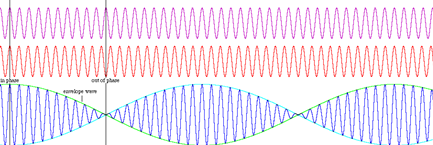
\includegraphics[]{images/widelane.png}
  \caption{Illustration of the linear widelane combinations. Two original frequencies (top and middle) are subtracted to form a longer wavelength observable (bottom)}%
  \label{fig:widelane}%
\end{figure*}



\subsection{Common widelane}
\begin{fullwidth}
To improve ambiguity resolution, often the wide lane linear combination (also called L5 or LW linear combination) is formed from the L1 and L2 carrier phase observables. It is designed to be a geometry-preserving combination using only carrier-phase measurements in the frequencies $f_a$ and $f_b$. By selecting the integer coefficients as $i_A = +1$ and $i_B = -1$, one obtains the WL carrier-phase combination $\phi_{r,WL}^s$ in units of cycles:
\end{fullwidth}
\begin{equation}
\phi_{r,WL}^s = \phi_{r,A}^A - \phi_{r,B}^S = \frac{\psi_{r,A}^s}{\lambda_A} - \frac{\psi{r,B}^s}{\lambda_B} \label{eq:wl_cycles}
\end{equation}

The corresponding wavelength $\lambda_{WL}$ is:
\begin{equation}
\lambda_{WL} = \frac{c}{f_A - f_B} 
    \label{eq:wl_wavelength}
\end{equation}

Multiplication of the two above equations leads to the wide-lane combination $\psi_{r,WL}^s$ in units of meters:
\begin{equation}
\psi_{r,WL}^S = \frac{f_A}{f_A-f_B}\psi_{r,A}^s - \frac{f_B}{f_A-f_B}\psi_{r,B}^s
\end{equation}

\subsection{Melbourne-Wubbena linear combination}
The Melbourne-Wubbena linear combination (Melbourne 1985),(Wubbena 1985) is a linear combination of the L1 and L2 carrier phase plus the P1 and P2 pseudorange. The geometry, troposphere and ionosphere are eliminated by it. The Melbourne-Wubbena linear combination can be represented as:

$
E(L_{r,IF}^S) - \frac{cf_2z_{r,w}^s}{f_1^2 - f_2^2} = \rho_r^s + c(dt_{r,IF} - dt_{IF}^s) + \tau_r^s + \lambda_n z_{r,1}^s + (\lambda_{IF}\delta_{r,IF}$

Since �!,,% comprises of both code and phase measurements, it is reasonable to exclude the lower
elevation measurements to avoid the multipath impacts from the code observation. Normally, with
30 degree elevation cut-off, an averaging of 5 minutes of (4) is good enough to fixing the wide-lane
ambiguities [RD 04]. The rests are the wide-lane phase bias, which can be broadcasted to the user for
user side wide-lane ambiguity resolution. Either choosing a pivot receiver bias or a single-differencing
between two satellites can avoid the linear dependency. 


-doesn't need lambda not as correlated